\subsubsection{Load Cell Calibration Study}

In order to maintain accurate thrust measurement within a test stand built for rotating detonation engines, the functionality of the test stand’s load cells is critical. In an ideal test stand configuration, the entirety of the thrust produced by the test article on the stand would be transferred through the load cells, measuring the thrust to an extremely accurate degree. However, due to the nature of balancing efficient force distribution with structurally stable test stand designs, it is impossible to obtain an exact force reading using the load cells.

To solve this issue, the load cells can be calibrated prior to each test, to determine the difference between the amount of thrust determined by the load cells and the actual thrust produced by the test article. The calibration process is one of the most important aspects to consider of test stand design, as an improper load cell calibration would lead to inaccurate or completely non-sensical thrust readings. This trade study focuses on the nature of the test stand’s load cell calibration structure, and different potential configurations that will minimize any inaccuracies that could occur during the calibration process.

\noindent\underline{Option 1: Hydraulic Calibration Structure}

A hydraulic calibration structure utilizes a rigid framework designed to integrate directly with the test stand, or in some instances, directly with the test article itself in order to calibrate the load cells. At its core, the system features a high-pressure hydraulic ram capable of applying precise and repeatable loads onto the test stand or test article, mimicking the forces at specific locations that would be seen during a testing campaign. The structure’s rigidity minimizes deflection and ensures that the applied force can be accurately transmitted to the load cell under test and is designed to handle the high forces that can be associated with the testing of rotating detonation engines, ensuring calibration under conditions closely resembling actual operational scenarios.

\begin{figure}
    \centering
    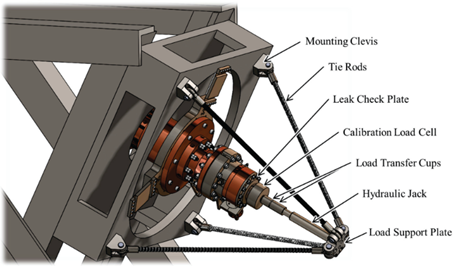
\includegraphics[width=0.6\linewidth]{hydraulic_calibration_example.png}
    \caption{An example of a hydraulic calibration structure developed by Purdue's Zucrow Labs.}
    \label{fig:hydraulic-calibration-example}
\end{figure}

\noindent\textit{Pros:}

If designed and assembled the right way, a hydraulic calibration structure would allow for exceptional accuracy and repeatability, which are critical for test stand applications. The hydraulic ram would be able to apply precise, controlled forces over a wide range, ensuring that the calibration data produced is highly reliable. With the incorporation of a rigid design, the deflection of the structure can be minimized, which helps to reduce measurement error as well. This precision makes the system suitable for higher-thrust applications where even minor inaccuracies could compromise data quality.

Another significant advantage of a hydraulic calibration structure is the system’s integration with the test stand and test article itself, ensuring that calibration occurs under realistic load conditions. By applying forces through the same paths and interfaces that will be used during actual tests, this method minimizes any structural differences that can occur between calibration and test configurations, such as misalignment or force path distortions. This approach results in a more accurate calibration, as it reflects the actual loading scenarios the load cells would experience during engine tests.

This structure also utilizes scalability and versatility to further enhance its utility. Hydraulic rams are capable of generating large amounts of force, which makes this design adaptable for calibrating a variety of load cells at different expected thrust amounts. Additionally, the ability to change the generated force of the hydraulic ram on the fly can allow precise calibration across the entire operational range of a load cell, ensuring accuracy across diverse test conditions. This flexibility can prove quite useful to testing campaigns looking to quickly iterate across different designs or setups.

\noindent\textit{Cons:}

One major drawback of the hydraulic calibration structure is its complexity and cost. The design and fabrication of a system capable of withstanding high forces without deflection demands significant resources. The hydraulic ram on its own could get quite expensive, in order to procure a ram that accurately provides the force required for an accurate load cell calibration. Additionally, the extra components required to mount the system to the test stand or test article can further add to the overall cost, as well as complexity required for the entire system to work.

Another limitation involves the significant setup and alignment time of the structure, which can lead to issues with operational delays. Ensuring proper alignment between the hydraulic ram, load cells, and calibration structure is crucial to avoid calibration errors, but this process can be fairly labor-intensive if designed poorly. Any issues that occur during setup can also introduce equipment errors or miscalibration of the hydraulic system itself, further adding to the overall calibration time.

This calibration structure also has the drawback of being unable to simulate dynamic or transient loads, which are critical for testing certain scenarios that could be experienced by the test article. While hydraulic systems excel at applying static forces, there is no efficient way to replicate any rapid thrust changes that could occur during a real-world testing campaign. This limitation could require the system to contain additional equipment in order to replicate these force conditions or ignore the calibration of dynamic thrust entirely.

\noindent\underline{Option 2: Mass-Pulley Calibration Structure}

A mass-pulley calibration structure involves attaching a mass pulley system to the test stand, with a procedure of applying known weights and measuring the resulting force read by the load cells. Specifically, a pulley would be placed on the back of the test stand, over which a string would be suspended below towards a platform in which the weights can be placed. Assuming the mass of the weights is exact, and the potential parasitic forces acting on the calibration system are known, the load cells in the test stand can be calibrated quite accurately.

\begin{figure}
    \centering
    \raisebox{-0.5\height}{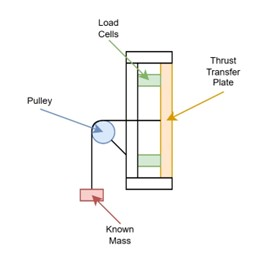
\includegraphics[width=0.4\linewidth]{mass-pulley-calibration-diagram.jpg}}
    \hspace{3em}
    \raisebox{-0.5\height}{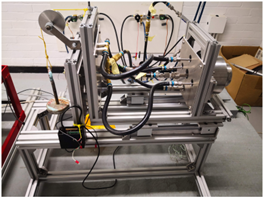
\includegraphics[width=0.4\linewidth]{mass-pulley-calibration-example.png}}
    \caption{\centering{A diagram of the pulley-and-weight calibration structure (left) and an example developed by the University of Southampton (right).}}
    \label{fig:mass-pulley-calibration-example}
\end{figure}

\noindent\textit{Pros:}

The use of a mass-pulley system for calibration is a lot more straightforward and cost-effective than most other solutions. It primarily relies on readily available components like calibrated weights, pulleys, and cables, making it easy to assemble and replicate. Any other required components would likely be able to be fabricated with ease as well. This simplicity reduces the potential for complex mechanical or electronic failures during the calibration process and ensures that the setup can be quickly adapted for different ranges of applied forces.

The mass-pulley calibration system is also much more well-suited for low-force ranges compared to high-force ranges. The accuracy with these lower forces means that the calibration system will be able to much more reliably measure thrust data closer to the range in which a standard small-scale rotating detonation engine will operate. Producing data in this critical range will allow the engine performance the be evaluated much more confidently.

Additionally, this calibration system’s modular design allows for much easier adjustments to the range of forces in which the load cells need to be calibrated to. Changing the force being applied to the load cell during the calibration process is as easy as adding to or changing the known weight being suspended below the pulley. This flexibility makes the structure suitable for a variety of thrust measurement scenarios, whether quickly calibrating between different iterations of a test article or between different expected thrusts that could be produced.

\noindent\textit{Cons:}

The use of a mass-pulley system for calibration is a lot more straightforward and cost-effective than most other solutions. It primarily relies on readily available components like calibrated weights, pulleys, and cables, making it easy to assemble and replicate. Any other required components would likely be able to be fabricated with ease as well. This simplicity reduces the potential for complex mechanical or electronic failures during the calibration process and ensures that the setup can be quickly adapted for different ranges of applied forces.

The mass-pulley calibration system is also much more well-suited for low-force ranges compared to high-force ranges. The accuracy with these lower forces means that the calibration system will be able to much more reliably measure thrust data closer to the range in which a standard small-scale rotating detonation engine will operate. Producing data in this critical range will allow the engine performance the be evaluated much more confidently.

Additionally, this calibration system’s modular design allows for much easier adjustments to the range of forces in which the load cells need to be calibrated to. Changing the force being applied to the load cell during the calibration process is as easy as adding to or changing the known weight being suspended below the pulley. This flexibility makes the structure suitable for a variety of thrust measurement scenarios, whether quickly calibrating between different iterations of a test article or between different expected thrusts that could be produced.

% ----- CRITERIA & WEIGHTS -----
\begin{table}[H]
    \centering
    \singlespacing
    \small
    \caption{Load Cell Calibration Trade Study - Evaluation Criteria}
    \label{tab:load_cell_calibration_eval_criteria}

    \begin{subtable}[t]{\linewidth}
        \begin{tabularx}{\linewidth}{
            |>{\hsize=0.200\hsize}>{\centering\arraybackslash}X
            |>{\hsize=0.100\hsize}>{\centering\arraybackslash}X
            |>{\hsize=0.700\hsize}>{\centering\arraybackslash}X|
        }
            \hline
            \textbf{Decision Criteria} & \textbf{Weight} & \textbf{Reason} \\ \hline

            Complexity & 15\% & The design needs to be able to achieve its goals without unnecessary complexity in its assembly, serviceability, or maintenance, that can yield extra failure modes or unexpected behavior. \\ \hline
        
            Manufacturability & 15\% & The test stand should be able to be machined at the UCF machine shop without added difficulty. \\ \hline
        
            Risk & 20\% & While each option being considered has been tested in research previously, their specific adaptation to SABR can and will introduce unexpected risks, making the configuration choice paramount. \\ \hline
        
            Technical Performance & 50\% & The design’s ability to reliably handle and accurately measure the thrust produced by SABR are crucial for the success of the project. \\ \hline
        \end{tabularx}
        \smallskip
        \caption{Evaluation Criteria and Weights}
    \end{subtable}

\end{table}

\vspace{-2em}

% ----- COMPLEXITY SCALE -----
\begin{table}[H]
    \centering
    \singlespacing
    \small
    \ContinuedFloat

    \begin{subtable}[t]{\linewidth}
        \begin{tabularx}{\linewidth}{
            |>{\hsize=0.150\hsize}>{\centering\arraybackslash}X
            |>{\hsize=0.850\hsize}>{\centering\arraybackslash}X|
        }
            \hline
            \textbf{Score} & \textbf{Reason} \\ \hline
        
            4 & Calibration involves minimal setup and few components, requiring basic tools or fixtures. \\ \hline
            
            3 & Calibration requires specialized equipment but remains relatively straightforward, the procedure involves multiple steps but is not resource intensive. \\ \hline
            
            2 & Calibration involves more advanced systems, requiring precise alignment and controlled environments. \\ \hline
            
            1 & Calibration uses dynamic or highly specialized systems and requires significant expertise. \\ \hline
        \end{tabularx}
        \smallskip
        \caption{Evaluation Scale - Complexity}
    \end{subtable}
\end{table}

\vspace{-2em}

% ----- MANUFACTURABILITY SCALE -----
\begin{table}[H]
    \centering
    \singlespacing
    \small
    \ContinuedFloat

    \begin{subtable}[t]{\linewidth}
        \begin{tabularx}{\linewidth}{
            |>{\hsize=0.150\hsize}>{\centering\arraybackslash}X
            |>{\hsize=0.850\hsize}>{\centering\arraybackslash}X|
        }
            \hline
            \textbf{Score} & \textbf{Reason} \\ \hline
        
            4 & The design uses standard components that require minimal customization, and any fabrication involves basic machining with minimal cost and lead times. \\ \hline
            
            3 & The design requires some custom components requiring some intermediate level machining but are not highly specialized or difficult to produce. \\ \hline
            
            2 & The design relies on custom-engineered parts or systems and requires more advanced techniques to fabricate. \\ \hline
            
            1 & The design incorporates highly specialized materials and would require extensive prototyping and specialized facilities. \\ \hline
        \end{tabularx}
        \smallskip
        \caption{Evaluation Scale - Manufacturability}
    \end{subtable}
\end{table}

\vspace{-2em}

% ----- RISK SCALE -----
\begin{table}[H]
    \centering
    \singlespacing
    \small
    \ContinuedFloat

    \begin{subtable}[t]{\linewidth}
        \begin{tabularx}{\linewidth}{
            |>{\hsize=0.150\hsize}>{\centering\arraybackslash}X
            |>{\hsize=0.850\hsize}>{\centering\arraybackslash}X|
        }
            \hline
            \textbf{Score} & \textbf{Reason} \\ \hline
        
            4 & The calibration process involves few safety or operational risks, and features simple, fail-safe mechanisms. \\ \hline
            
            3 & The calibration process involves some operational risks, but they are manageable with standard precautions. Safety concerns can be easily mitigated through training. \\ \hline
            
            2 & The calibration process involves significant operational risks, and safety hazards requiring strict protocols and regular maintenance exist. \\ \hline
            
            1 & The calibration process involves highly complex components with catastrophic failure modes. System failure could lead to severe safety incidents or irreparable damage. \\ \hline
        \end{tabularx}
        \smallskip
        \caption{Evaluation Scale - Risk}
    \end{subtable}
\end{table}

\vspace{-2em}

% ----- TECHNICAL PERFORMANCE SCALE -----
\begin{table}[H]
    \centering
    \singlespacing
    \small
    \ContinuedFloat

    \begin{subtable}[t]{\linewidth}
        \begin{tabularx}{\linewidth}{
            |>{\hsize=0.150\hsize}>{\centering\arraybackslash}X
            |>{\hsize=0.850\hsize}>{\centering\arraybackslash}X|
        }
            \hline
            \textbf{Score} & \textbf{Reason} \\ \hline
        
            4 & The design exceeds the desired thrust measurement requirements for SABR performance. \\ \hline
            
            3 & The design meets the minimum thrust measurement requirements for SABR performance. \\ \hline
            
            2 & The design can meet the minimum thrust measurement requirements for SABR performance but requires a significant amount of post-processing on the load cell data. \\ \hline
            
            1 & The design is inefficient, ineffective, or otherwise fails to meet the desired thrust measurement requirements for SABR. \\ \hline
        \end{tabularx}
        \smallskip
        \caption{Evaluation Scale - Technical Performance}
    \end{subtable}
\end{table}

\vspace{-2em}

% ----- DECISION MATRIX -----
\begin{table}[H]
    \centering
    \singlespacing
    \small
    \begin{tabularx}{0.8\linewidth}{
        |>{\hsize=0.35\hsize}>{\centering\arraybackslash}X
        |>{\hsize=0.15\hsize}>{\centering\arraybackslash}X
        |>{\hsize=0.25\hsize}>{\centering\arraybackslash}X
        |>{\hsize=0.25\hsize}>{\centering\arraybackslash}X|
    }
        \hline
        \multicolumn{2}{|c|}{\textbf{Criteria and Weights}} & \multicolumn{2}{|c|}{\textbf{Options and Scores}} \\ \hline

        \textbf{Criteria} & \textbf{Weights} & \textbf{Hydraulic Calibration Structure} & \textbf{Mass-Pulley Calibration Structure} \\ \hline

        \multicolumn{1}{|l|}{\textbf{Complexity}} & 0.25 & 3 & 4 \\ \hline

        \multicolumn{1}{|l|}{\textbf{Manufacturability}} & 0.15 & 2 & 4 \\ \hline

        \multicolumn{1}{|l|}{\textbf{Risk}} & 0.10 & 3 & 4 \\ \hline

        \multicolumn{1}{|l|}{\textbf{Technical Performance}} & 0.50 & 4 & 3 \\ \Xhline{2pt}

        \multicolumn{2}{|l|}{\textbf{Weighted Scores}} & \textbf{3.35} & \textbf{3.50} \\ \hline
        
    \end{tabularx}
    \caption{Load Cell Calibration Trade Study - Decision Matrix}
    \label{tab:load_cell_calibration_decision_matrix}
\end{table}

\noindent\underline{Decision}

As shown by the decision matrix, a mass-pulley system is the ideal choice for the test stand calibration structure. It is less complex in its design, much easier to manufacture, and slightly less risky than the option of a hydraulic calibration structure, but slightly less accurate in its ability to calibrate to a high enough accuracy. Despite the lower accuracy, the mass-pulley system is still more than capable of meeting the minimum project requirements, and its shortcomings are easily outweighed by its lack of complexity and cost. On the other hand, the use of the hydraulic calibration structure would likely yield load cell calibration to a higher accuracy, but with the drawbacks of a much more complex and risky system.